\chapter{Parallelism}
\section{Motivation}
\begin{definitionbox}{Denbard/MOSFET Scaling}
    A scaling/power law stating that as transistors get smaller:
    \begin{itemize}
        \item Power density is constant, hence power $\varpropto$ area.
        \item Voltage and current decrease with transistor length.
    \end{itemize}
    Hence as transistor size decreases they become faster, more energy efficient and cheaper.
    \begin{itemize}
        \item Part of a \href{https://ieeexplore.ieee.org/document/1050511}{paper} (1974) on MOSFETs (metal-oxide-semiconductor field-effect transistors) co-authored by Robert Dennard
        \item Scaling becomes limited by transistor leakage, which grows as a proportion of power consumed by the transistor as scale is decreased.
        \item Leakage converts to heat which must be dissipated to prevent damage to the chip. This presents a limiting factor on scaling.
    \end{itemize}
\end{definitionbox}
\noindent
Slow end of \textit{Dennard scaling} limit single threaded performance improvements $\Rightarrow$ Increase parallelism to attain higher performance.

\begin{definitionbox}{Ambdahl's Law}
    Where $S$ is speedup, and each $p_i, s_i$ is the speedup for a proportion of the program.
    \[S = \left(\cfrac{p_1}{s_1} + \cfrac{p_2}{s_2} + \dots + \cfrac{p_n}{s_n}\right)^{-1}\]
    We can simplify this for the basic case of proportion $p$ of a program perfectly parallelised over $n$ threads:
    \[S = \cfrac{1}{(1-p) + \cfrac{p}{n}}\]
\end{definitionbox}

\subsection{Types of Parallelism}
\begin{definitionbox}{Data-Level Parallelism}
    Increasing throughput by operating on multiple elements of data in parallel.
    \\
    \\ Typically this in the form of \textbf{S}ingle-\textbf{I}nstruction \textbf{M}ultiple-\textbf{D}ata 
    (\textbf{SIMD}) instruction-set extension (instructions that operate a single simple instruction on several 
    (typically adjacent) data elements. 
    \\
    \\ Some such extensions include:
    \vspace{2mm}
    \\ \begin{tabular}{l p{.9\textwidth}}
        \textbf{MMX} & An early \textbf{SIMD} instruction set extension for IA32 developed by Intel for the Pentium P5 microarchitecture (1997), only supports integer arithmetic. \\
        \textbf{SSE} & (\textbf{S}treaming \textbf{S}IMD \textbf{E}xtensions) developed by Intel that support floating point arithmetic. \\
        \textbf{AVX} & (\textbf{A}dvanced \textbf{V}ector \textbf{E}xtensions) developed by Intel and AMD for x86-64 (Sandy bridge \& AMD Bulldozer IN 2011). \\
    \end{tabular}
    \vspace{2mm}
    \\ Another form is \textbf{S}ingle-\textbf{I}nstruction \textbf{M}ultiple-\textbf{T}hreads (\textbf{SIMT}) where each thread operates on some data, and many threads execute the same instructions in lockstep. This is the programming model used by most GPUs (e.g see Nvidia's CUDA).
\end{definitionbox}

\begin{definitionbox}{Instruction Level Parallelism}
    Systems where multiple instructions can be executed in the same step (e.g instructions per cycle $> 1$). Many techniques are used to achieve this:
    \vspace{2mm}
    \\ \begin{tabular}{l p{.8\textwidth}}
        \textbf{Pipelining} & Allows higher throughput by splitting an instruction pipeline into stages that can be executed in parallel. \\
        \textbf{VLIW} \& \textbf{EPIC} & (\textbf{V}ery-\textbf{L}ong \textbf{I}nstruction \textbf{W}ord \& \textbf{E}xplicitly \textbf{P}arallel \textbf{I}nstruction \textbf{C}omputing) architectures where instructions contain bundles of operations and explicitly determine which operations can be run in parallel (e.g Intel's Itanium/IA64). It is a way for statically scheduled processors to take advantage of ILP, but is not common. \\
        \textbf{Superscalar} & Dynamically scheduled processors that can inspect instruction dependencies at runtime in order to dispatch fetched instructions for execution out-of-order and in parallel. Many other techniques can be used here such as speculative execution and register renaming. \\
    \end{tabular}
    Nearly all modern processors are pipelined \& superscalar.
\end{definitionbox}

\begin{sidenotebox}{Flynn's Taxonomy}
    A classification scheme for computer architectures that neatly describes the type of parallelism they use (see wikipedia \href{https://en.wikipedia.org/wiki/Flynn%27s_taxonomy}{here}).
\end{sidenotebox}

\begin{definitionbox}{Task-Level Parallelism}
    Splitting an algorithm into sections that can be run in parallel.
    \begin{itemize}
        \item Parallelism must be extracted by the programmer.
        \item Tasks run in separate processes or threads, potentially on different cores, or processors. 
        \item Each task being run in parallel can be different (different instructions and either different data or shared data accessed)
    \end{itemize}
\end{definitionbox}

\begin{sidenotebox}{Crazy Fast IPC}
    The L4 microkernel implements \textit{short IPC} where a sending process places the message in registers, and a fast context switch to the receiving thread without clearing registers (explained \href{https://os.itec.kit.edu/downloads/sa_2002_wenske-horst_fast-local-ipc.pdf}{here}).
    \\
    \\ The L4ka project at Karlsruher University's Operating Systems group has an Itanium implementation that takes advantage of this (and Itanium specifics $\to$ lots of registers) to complete short IPC in as few as \href{https://www.cs.hs-rm.de/~kaiser/2020_aos/05b-ukx6.pdf}{$36$ cycles}.
\end{sidenotebox}

\subsection{Concurrency}
\begin{center}
    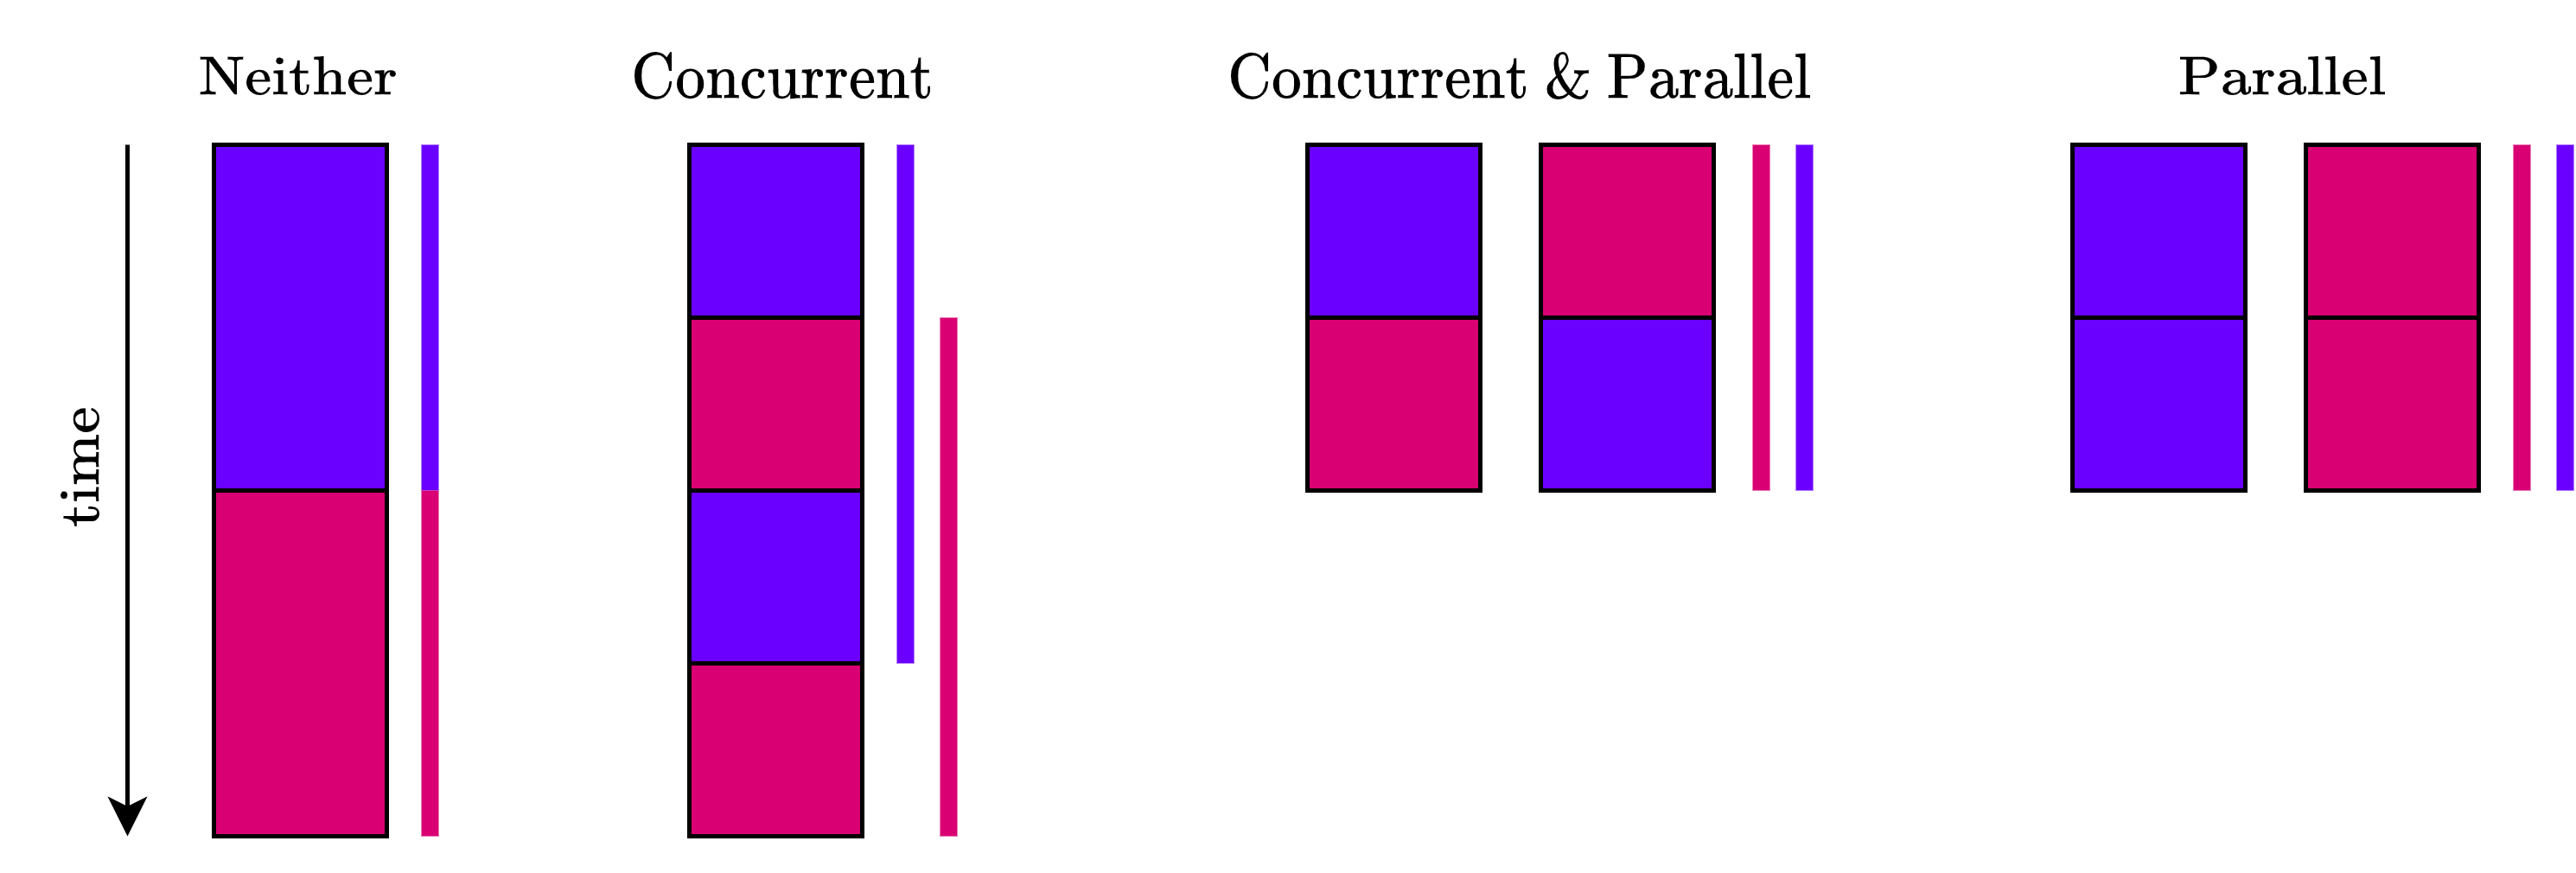
\includegraphics[width=.8\textwidth]{parallelism/images/concurrent_vs_parallel.drawio.png}
\end{center}
\begin{tcbraster}[raster columns=2,raster equal height]
\begin{definitionbox}{Parallel}
    \textit{"Decomposing a problem into smaller tasks executed at the same time on different compute resources"}
\end{definitionbox}
\begin{definitionbox}{Concurrent}
    \textit{"Decomposing a problem into smaller tasks executed during overlapping time periods"}
\end{definitionbox}
\end{tcbraster}
\begin{center}
    \begin{tabular}{r r p{.7\textwidth}}
        $\mathcal{C}$ & $\neg \mathcal{P}$ & An OS scheduler interleaving the execution of two threads on a core. \\
        $\mathcal{C}$ & $\mathcal{P}$      & Threads switching cores (OS scheduler typically tries to avoid this). \\
        $\neg \mathcal{C}$ & $\mathcal{P}$ & Two threads executed entirely on separate cores. \\
    \end{tabular}
\end{center}

\subsection{Cost Efficiency}
\begin{examplebox}{What is it good for!}
    What are the main advantages of parallelism?
    \tcblower
    \begin{itemize}
        \item Better performance through parallelism
        \item Better cost-efficiency (can share RAW, disk, network cards between several cores, rather than needing separate machines)
    \end{itemize}
    Much of this is workload and algorithm specific $\to$ a user needs to analyze their specific use case to determine the appropriate hardware.
\end{examplebox}
Datacenters optimise for \textit{total cost of ownership}:
\begin{itemize}
    \item Entire hardware lifecycle (purchase, expected maintenance, mean time-to-failure).
    \item Energy consumption \& cooling requirements.
    \item land, building \& even security costs.
    \item Existing hardware compatibility.
\end{itemize}

\begin{examplebox}{CPU provisioning}
    Given the following specifications:
    \begin{itemize}
        \item 1 Gbps network
        \item Requests are 1KB
        \item Each requet takes 50$\mu$s to process
    \end{itemize}
    \tcblower
    \[\underbrace{2^{30}}_{\text{1 Gbps Network}}  \div \underbrace{2^3}_{8 \ bits = 1 \ byte} \div \underbrace{2^10}_{\text{1 KB request}} = 2^{17} \ \text{ requests per second}\]
    Each core can process a request in $50\mu s$ so:
    \[(50 \times 10^{-6})^{-1} = (5 \times 10^{-5})^{-1} = 2 \times 10^4 \ \text{ requests per second}\]
    Hence to saturate the flow of incoming requests:
    \[cores = \left\lceil \cfrac{requests / sec}{requests / sec / core} \right\rceil = \left\lceil \cfrac{2^{17}}{2 \times 10^4} \right\rceil \approx \lceil 6.5 \rceil = 7\]
\end{examplebox}

\subsection{Critical Path Analysis}
\begin{definitionbox}{Critical Path}
    A sequence of tasks determining the minimum time for an operation.
    \begin{center}
        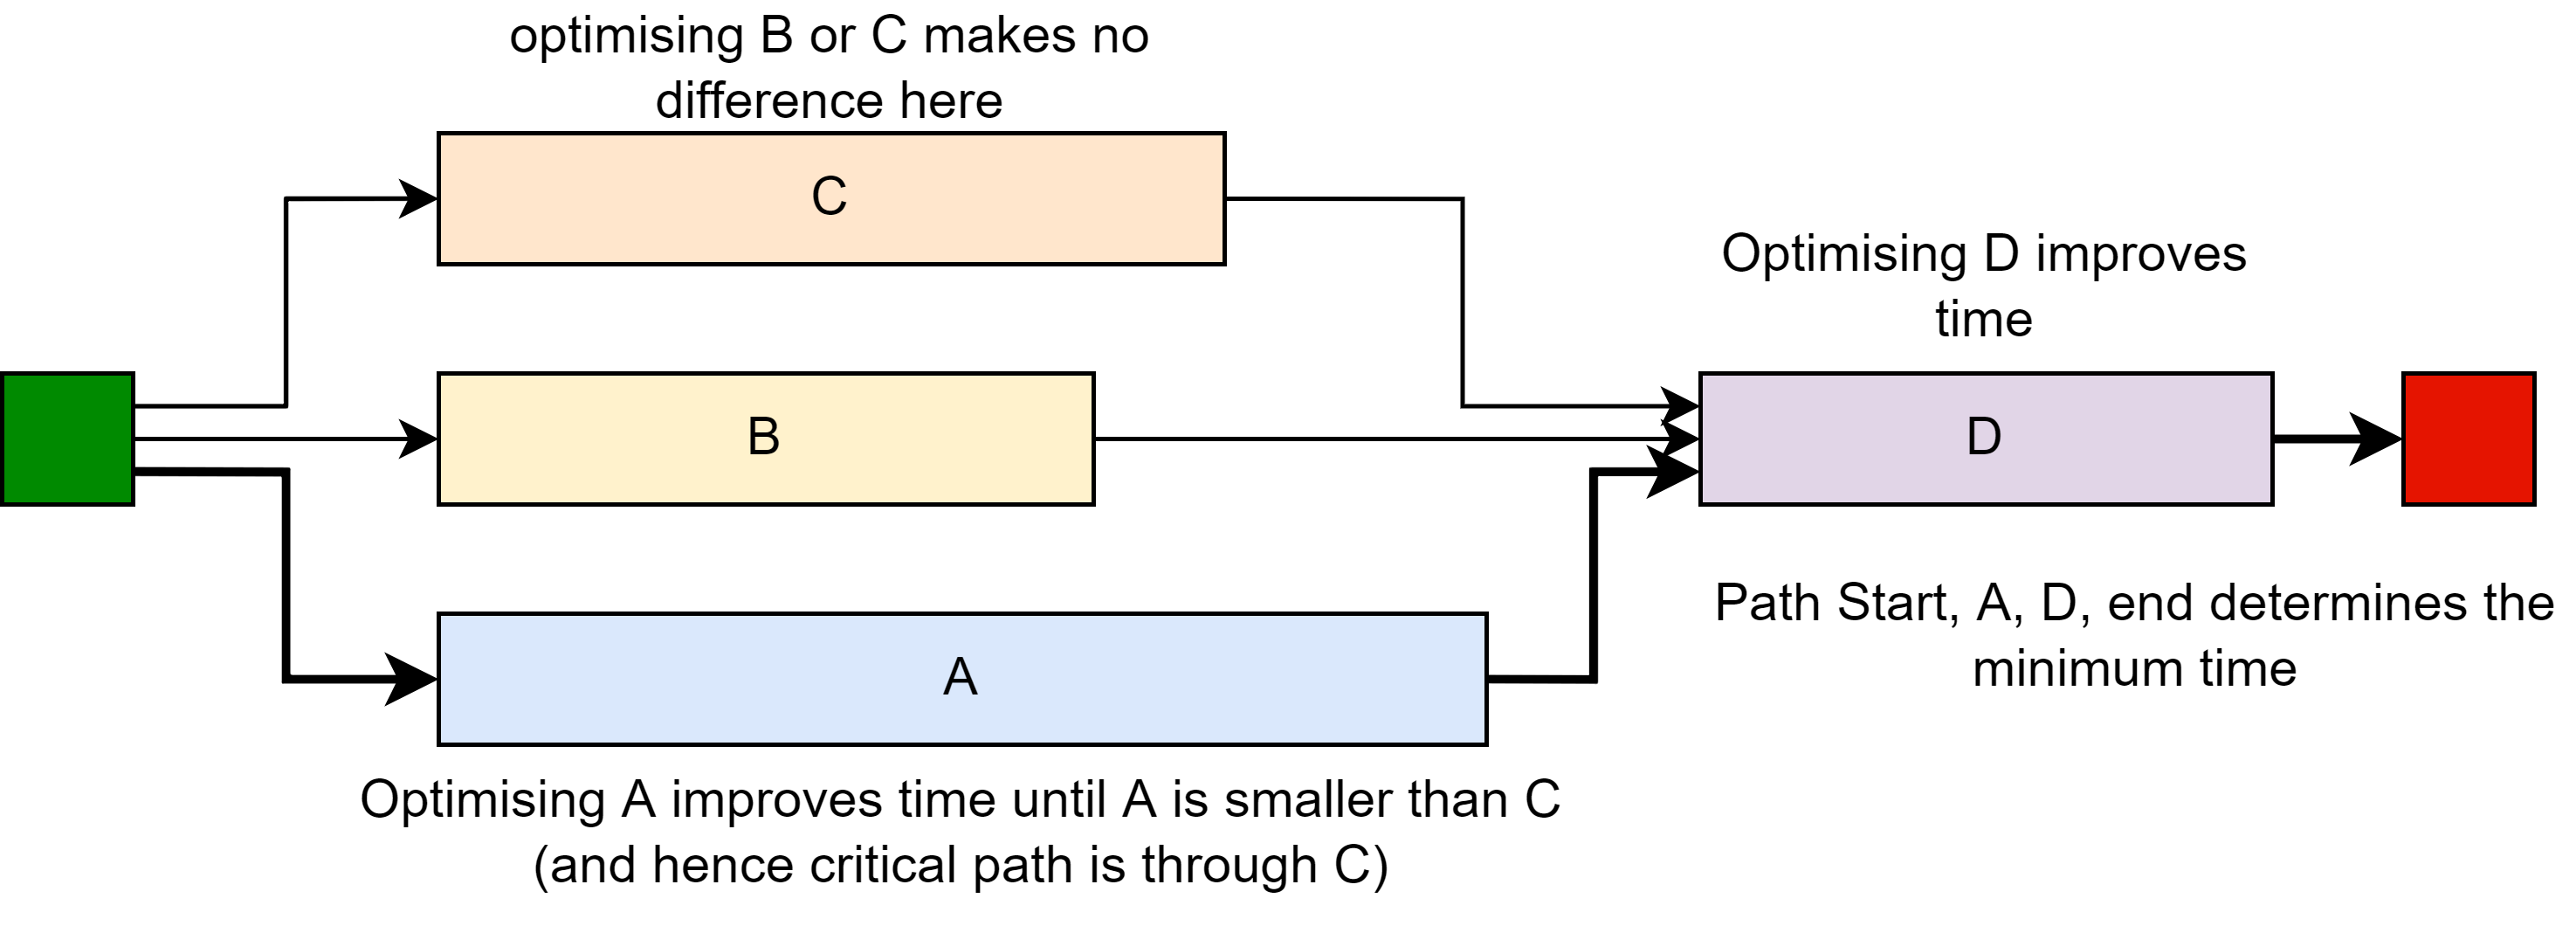
\includegraphics[width=.8\textwidth]{parallelism/images/critical_path.drawio.png}
    \end{center}
    \begin{itemize}
        \item The profiler is unaware of the critical path across threads (open area of research)
        \item Optimising outside of the critical path will often not improve time.
    \end{itemize}
\end{definitionbox}


\section{Cache Coherency}
CPUs contain multiple levels of data caches (L1, L2, L3/LLC) which need to be coherent (same cached location $\Rightarrow$ same value).
\\
\\ A cache coherency protocol determines how a CPU achieves this. Typically each cache line has some state, with the protocol determining how and when cache lines transition state depending on issues reads and writes.
\\
\\ MSI is a simple cache coherency algorithm.

% Slides dont show entire MSI => wikipedia is good, but is it assessed?

\unfinished

In order to add support for atomics and additional \textbf{Locked} state is included

\section{Atomics}
Atomic read, modify and write operations require hardware support and are exposed
 to programmers through compiler supported libraries (e.g stdatomic for C11, C++ \href{https://en.cppreference.com/w/cpp/atomic}{atomic} and Rust \href{https://doc.rust-lang.org/std/sync/atomic/}{\mintinline{rust}{std::sync::atomic}}).

\begin{sidenotebox}{Lock Prefix}
    The IA32 \& x86-64 support a \mintinline{asm}{lock} prefix for some instructions to specify they should be run atomically. 

\begin{minipage}[t]{.55\textwidth}
    \inputminted{c}{parallelism/code/cmpxchg.c}
\end{minipage}
\begin{minipage}[t]{.45\textwidth}
    \inputminted{asm}{parallelism/code/cmpxchg.s}
\end{minipage}
\end{sidenotebox}

Atomic methods often allow the programmer to specify the memory order (order of memory accesses around the atomic access).
\begin{minted}{cpp}
enum class memory_order : /* unspecified */ {
    relaxed, // relaxed ordering - no guarantee on ordering
    consume, // release-consume ordering
    acquire, // release-acquire ordering
    release, // release-acquire and release-consume ordering 
    acq_rel, // both release and acquire
    seq_cst  // sequentially consistent ordering
};
\end{minted}
These orders are well-documented \href{https://en.cppreference.com/w/cpp/atomic/memory_order}{here on cppreference}. 

\section{Synchronisation}
\subsection{Synchronisation Primitives}
\begin{tcbraster}[raster columns=2,raster equal height]
    \begin{definitionbox}{Mutex/Lock}
        Can only be held by one thread, blocks otherwise. Single thread in critical region.
        \tcblower
        \mintinline{cpp}{std::mutex}
    \end{definitionbox}
    \begin{definitionbox}{Shared Mutex/RW Lock}
        A mutex with a shared and exclusive lock.
        Allows any number of \textit{readers} or single \textit{writer} into a critical region.
        \tcblower
        \mintinline{cpp}{std::shared_mutex}
    \end{definitionbox}
    \begin{definitionbox}{Semaphore}
        Can be incremented/decremented, waits until value is $> 0$. 
        Allows $n$ threads into a critical region.
        \tcblower
        \mintinline{cpp}{std::counting_semaphore}
        \\ \mintinline{cpp}{std::binary_semaphore}
    \end{definitionbox}
    \begin{definitionbox}{Condition Variable}
        Set threads to wait until a condition is signalled as true (can use predicates, or have threads signal to wake up $n$ waiting threads).
        \tcblower
        \mintinline{cpp}{std::condition_variable} 
    \end{definitionbox}
\end{tcbraster}
\begin{definitionbox}{Barrier}
    Forces $n$ threads reaching the barrier to wait, until $n$ have arrived, at which point all are unblocked.
    \tcblower
    \mintinline{cpp}{std::barrier}
\end{definitionbox}

\subsection{Lock Implementation}
\subsubsection{User-Space}
Must make use of atomics to create spinlocks.
\begin{itemize}
    \item Basic locks just use CAS to wait on a flag.
    \item Intrinstics such as \mintinline{cpp}{_mm_pause()} can be used to wait efficiently (produces no-ops)
    \item Backoff (fixed \& exponential) can be used to decrease contention in access to the lock's flag.
    \item Other spinlock types such as ticket locks can add guarantees in order of acquisition by threads. 
\end{itemize}

\begin{tabbox}{prosbox}
    \textbf{No Kernel} & No kernel involvement means potentially less overhead when contention is low. \\
\end{tabbox}

\begin{tabbox}{consbox}
    \textbf{Spinning} & Waiting threads consume valuable CPU resources while spinning. This can become a severe issue if the spinning thread has higher priority than the thread holding the lock. \\
    \textbf{Starvation} & For a basic thread implementation there is no ordering on acquisition, so a thread may be constantly skipped/other threads that more recently attempted acquire the lock.  (Note: ticket locks guarantee this ordering) \\ 
\end{tabbox}

\subsubsection{Kernel Level Lock}
Lock and unlock via a syscall, with logic implemented in kernel space. If a thread cannot acquire the lock, thens schedule another thread.  
\begin{itemize}
    \item Can implement same CAS based acquisition attempt within the kernel (multiple threads on multiple cores may be servicing a syscall simultaneously)
    \item In systems with a single hardware thread, mutual exclusion within the kernel can be achieved by disabling interrupts (e.g as in Pintos, not possible on modern systems)
\end{itemize}

\begin{tabbox}{prosbox}
    \textbf{Fairness} & Can keep a queue of blocked/waiting threads and wake them in order. \\ 
\end{tabbox}
\begin{tabbox}{consbox}
    \textbf{Expensive} & If the lock is released/available, then acquisition has the additional overhead of a syscall when compared to a user level implementation. \\ 
\end{tabbox}

\subsubsection{Hybrid Level Lock}
A user level lock that bails out to a kernel level list of blocked waiters when contention is high.
\begin{itemize}
    \item Most popular implementation is the linux \textit{futex} (\textit{fast userspace mutex}).
    \item \mintinline{c}{pthread_mutex_lock} uses a futex internally
\end{itemize}

\begin{tabbox}{prosbox}
    \textbf{Adaptable} & Can dynamically adapt to spin in userspace, or block from kernel based on contention at runtime. \\  
\end{tabbox}

\section{False Sharing}
\begin{center}
    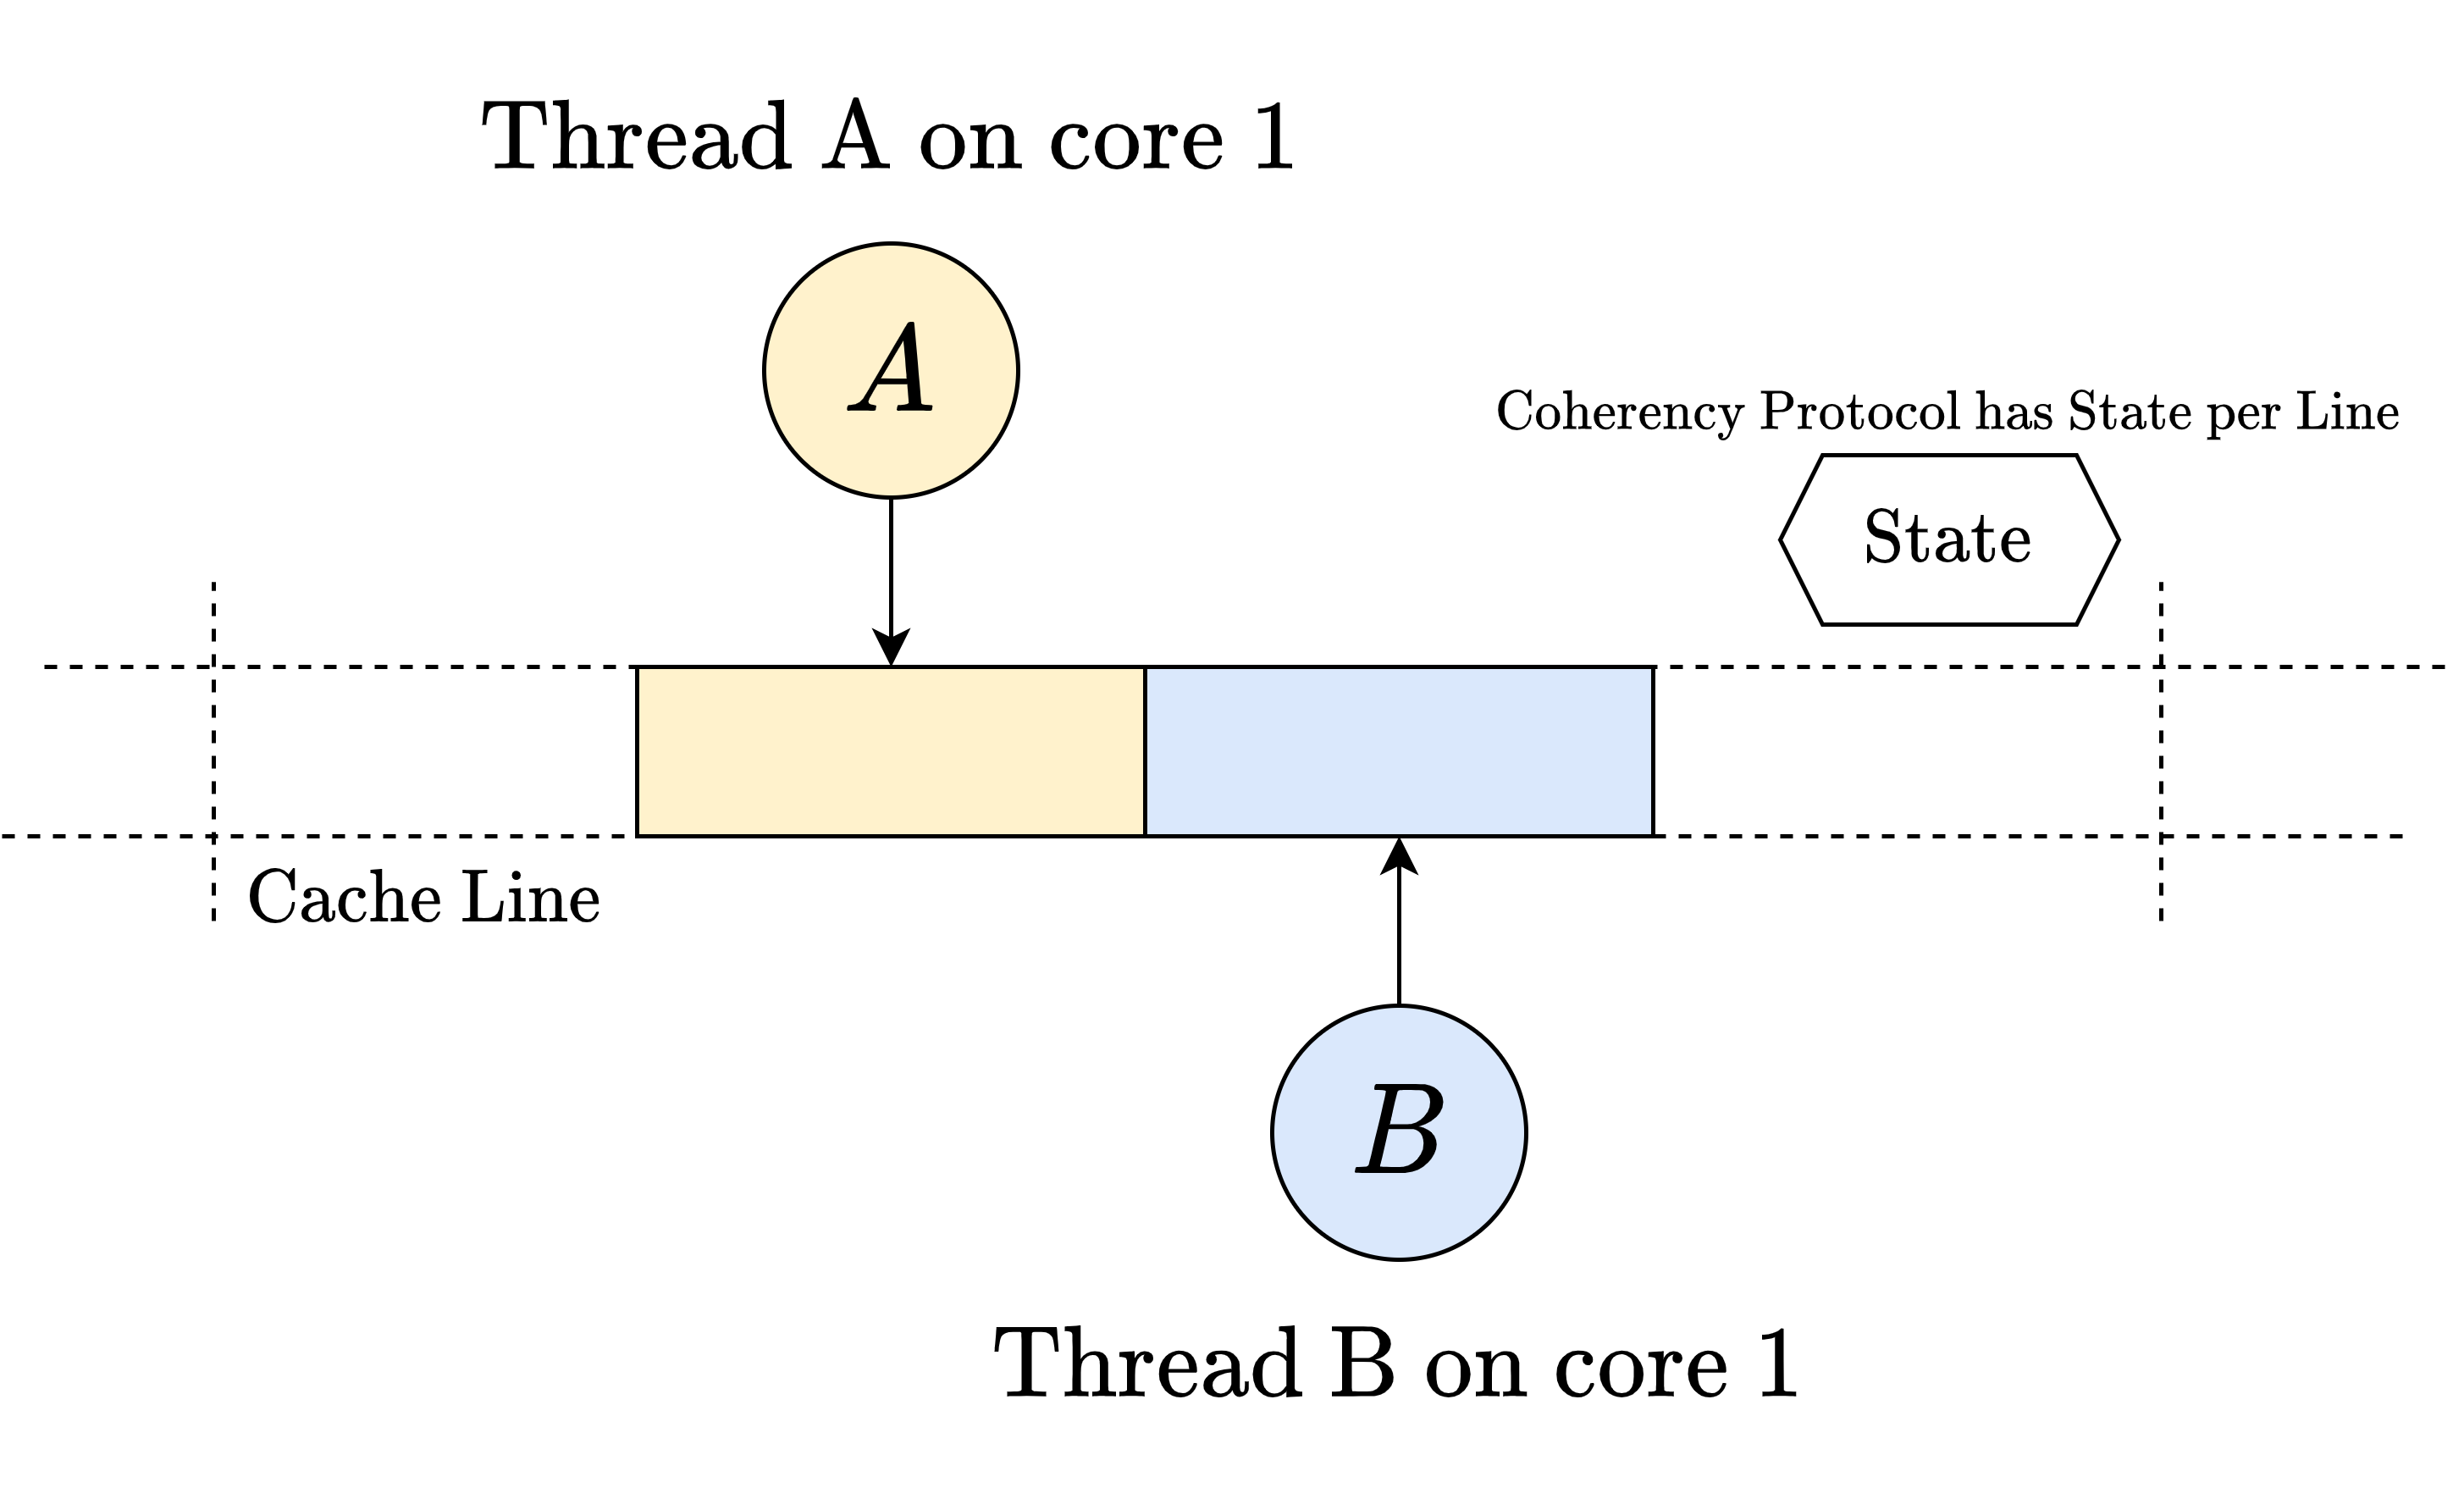
\includegraphics[width=.7\textwidth]{parallelism/images/false_sharing.drawio.png}
\end{center}
Cache coherency protocols store state per line. Multiple threads may not access shared data, but may access locations in that map to the same cache lines and if any threads write the line may be continually invalidated.
\begin{itemize}
    \item We can use hardware counters (e.g profiling with perf, using the HITM (hit modified) counter on x86-64 CPUs) to find false sharing occuring.
\end{itemize}

\section{Distributing Work}
We can implement some basic work distribution schemes using a Task.
\begin{minted}{cpp}
struct Task {
  virtual void run() = 0;
};

// We can make use of std::reference_wrapper to pass references to a polymorphic task type
using TaskRef = std::reference_wrapper<Task>;
using TaskQueue = std::vector<TaskRef>;
\end{minted}
\begin{itemize}
    \item Virtual method allows for polymorphism in tasks
    \item Task can store state, and return values.
\end{itemize}
We will make use of some example tasks:
\\ \begin{minipage}[t]{.49\textwidth}
    \begin{minted}{cpp}
struct PrintTask : Task {
  int id;

  PrintTask(int id) : id(id) {
    std::cout << "Created PrintTask: " 
              << id 
              << std::endl;
  }

  void run() override { 
    std::cout << "PrintTask: " 
              << id 
              << std::endl;
  }
};
    \end{minted}
\end{minipage}
\hfill \begin{minipage}[t]{.49\textwidth}
    \begin{minted}{cpp}
struct WaitTask : Task {
  int id;
  std::chrono::milliseconds wait_ms;

  WaitTask(int id, int waitfor) 
    : id(id), wait_ms(waitfor) {
    std::cout << "Created WaitTask: " 
              << id 
              << std::endl;
  }

  void run() override {
    std::cout << "started WaitTask: " 
              << id 
              << std::endl;
    std::this_thread::sleep_for(wait_ms);
    std::cout << "Ended WaitTask: " 
              << id 
              << std::endl;
  }
};
    \end{minted}
\end{minipage}
Runnable through a function for each work distribution:
\begin{minted}{cpp}
int main() {
  /* Can allocate tasks on stack, in a vector, etc */
  PrintTask a(0); PrintTask b(1); PrintTask c(2); PrintTask d(3);

  /* Create a task Queue to pass to method */
  TaskQueue tasks{a, b, c, d};

  auto start = std::chrono::steady_clock::now();

  /* Run tasks (comment out all but one method) */
  process_sequential   (tasks);
  process_on_demand    (tasks);
  process_fork_and_join(tasks);
  process_dispatch     (tasks);
  process_jobsteal     (tasks);

  auto end = std::chrono::steady_clock::now();
  
  /* Display time */
  std::cout << "Time: " << (end - start).count() << std::endl;
}
\end{minted}
\subsection{Sequential}
\begin{minted}{cpp}
void process_sequential(TaskQueue &tasks) {
  for (auto &task : tasks) {
    task.get().run();
  }
}   
\end{minted}
\begin{tabbox}{prosbox}
    \textbf{Simple} & No reasoning about concurrency required, easy to implement \& understand performance. \\
    \textbf{Low Overhead} & No overhead for using synchronisation primitives, as required by concurrent schemes. \\
\end{tabbox}
\begin{tabbox}{consbox}
    \textbf{No Parallelism}
\end{tabbox}

\subsection{On Demand}
\begin{minted}{cpp}
// Invariant: tasks' lifetime > threads (threads reference tasks)
void process_on_demand(TaskQueue &tasks) {
  std::vector<std::thread> threads;
  for (auto &task : tasks) {
    std::thread([&]() { task.get().run(); }).detach();
  }
}
\end{minted}
\begin{tabbox}{prosbox}
    \textbf{Simple} & Each thread only accesses task once, all synchronisation after is part of the task. \\
\end{tabbox}
\begin{tabbox}{consbox}
    \textbf{Performance} & Spawning threads is expensive, and when there is a large number of threads (e.g when os threads $>$ hardware threads) scheduling and contention on locks protecting shared data accessed by tasks reduce performance. \\
\end{tabbox}

\subsection{Fork \& Join}
For each batch of tasks, spawn new threads.
\begin{minted}{cpp}
void process_fork_and_join(TaskQueue &tasks) {
  std::vector<std::thread> threads;
  for (auto &task : tasks) {
    threads.emplace_back(std::thread([&]() { task.get().run(); }));
  }
  for (auto &thread : threads) {
    thread.join();
  }
}
\end{minted}
\begin{sidenotebox}{OpenMP}
    OpenMP is a set of standards for adding high-level parallelism directives into multiple languages (Fortran, C and C++).
    \href{https://www.openmp.org/wp-content/uploads/OpenMPRefCard-5-2-web.pdf}{OpenMP references}
    \begin{minted}{cpp}
#pragma omp for
for ( /* ... */ ) { 
    /* block executed in parallel  with other iterations */ 
}
    \end{minted}
\end{sidenotebox}

\subsection{Work Dispatching}
Each worker has its own queue, tasks are dispatched to each queue.
\begin{itemize}
    \item Queue is accessed by a main thread and a single worker
    \item Fixed number of workers
\end{itemize}
\begin{minted}{cpp}
struct WorkerQueue {
  WorkerQueue() : finish_(false), worker_([&]() {
    while (!finish_.load()) {
      auto task = get_task();
      if (task.has_value()) task.value().get().run();
    }
  }) {}

  void add_task(TaskRef task) {
    const std::lock_guard<std::mutex> lock(tasks_mutex_);
    tasks_.push_front(task);
  }

  std::optional<TaskRef> get_task() {
    const std::lock_guard<std::mutex> lock(tasks_mutex_);
    if (!tasks_.empty()) {
      auto task = tasks_.back();
      tasks_.pop_back();
      return task;
    } else { return {}; }
  }

  size_t size() const {
    const std::lock_guard<std::mutex> lock(tasks_mutex_);
    return tasks_.size();
  }

  void finish() {
    finish_.store(true);
    worker_.join();
  }

private:
  mutable std::mutex tasks_mutex_;
  std::deque<TaskRef> tasks_;
  std::atomic<bool> finish_;
  std::thread worker_;
};
\end{minted}
We can then create a pool of \mintinline{cpp}{WorkerQueue}s and allocate tasks in a round-robin scheme.
\begin{minted}{cpp}
template <size_t THREADS> struct WorkerPool {
  WorkerPool() : task_number_(0) {}

  void push_task(TaskRef task) {
    size_t index = task_number_.fetch_add(1) % THREADS;
    queues_[index].add_task(task);
  }

  void finish() {
    for (auto &q : queues_)
      q.finish();
  }

private:
  std::array<WorkerQueue, THREADS> queues_;
  std::atomic<size_t> task_number_;
};
\end{minted}

\begin{minted}{cpp}
void process_dispatch(TaskQueue &tasks) {
  WorkerPool<5> workerPool;
  for (auto t : tasks) {
    workerPool.push_task(t);
  }
  workerPool.finish();
}
\end{minted}
\begin{sidenotebox}{Improve these examples!}
    These examples have threads spin until a job is found, to improve efficiency we could suspend threads while no tasks are present.
    \begin{itemize}
        \item Could use a semaphore (\mintinline{cpp}{#include <semaphore>} from C++20 (only available in newer versions of GCC)).
        \item Need to ensure that suspended threads are still ended when \mintinline{cpp}{WorkerQueue::finish} is called.
        \item Could use a condition variable to implement producer-consumer pattern with finish.
    \end{itemize}
\end{sidenotebox}

\begin{tabbox}{prosbox}
    \textbf{Contention} & Each thread has its own queue, and hence can only contend for access with the thread/threads adding to the queue, not other workers. \\
\end{tabbox}
\begin{tabbox}[.7\textwidth]{consbox}
    \textbf{Consumer Balancing} & Some threads may finish jobs quickly and idle, while others are still completing work, but the tasks may still be allocated to busy threads.
\end{tabbox}
\subsection{Work Stealing}
Many threads contend to take tasks from a queue.
\begin{minted}{cpp}
template <size_t THREADS> struct TaskPool {
  TaskPool() : finish_(false) {
    for (auto &t : threads_)
      t = std::thread([&]() {
        while (!finish_.load()) {
          tasks_mutex_.lock();
          if (!tasks_.empty()) {
            TaskRef task = tasks_.back();
            tasks_.pop_back();
            tasks_mutex_.unlock();
            task.get().run();
          } else {
            tasks_mutex_.unlock();
          }
        }
      });
  }

  void submit_task(TaskRef task) {
    const std::lock_guard<std::mutex> lock(tasks_mutex_);
    tasks_.push_front(task);
  }

  size_t size() const {
    const std::lock_guard<std::mutex> lock(tasks_mutex_);
    return tasks_.size();
  }

  void finish() {
    finish_.store(true);
    for (auto &t : threads_)
      t.join();
  }

private:
  std::mutex tasks_mutex_;
  std::deque<TaskRef> tasks_;
  std::array<std::thread, THREADS> threads_;
  std::atomic<bool> finish_;
};
\end{minted}
\begin{minted}{cpp}
void process_jobsteal(TaskQueue &tasks) {
  TaskPool<5> taskpool;
  for (auto t : tasks) {
    taskpool.submit_task(t);
  }
  taskpool.finish();
}
\end{minted}

\begin{tabbox}{prosbox}
    \textbf{Consumer Balancing} & Tasks are \textit{stolen} by idle threads, busy threads are not overloaded with tasks. \\
\end{tabbox}
\begin{tabbox}{consbox}
    \textbf{Contention} & All threads waiting for new jobs contend for access to the same queue. \\
\end{tabbox}

\subsection{Streaming}
\begin{center}
    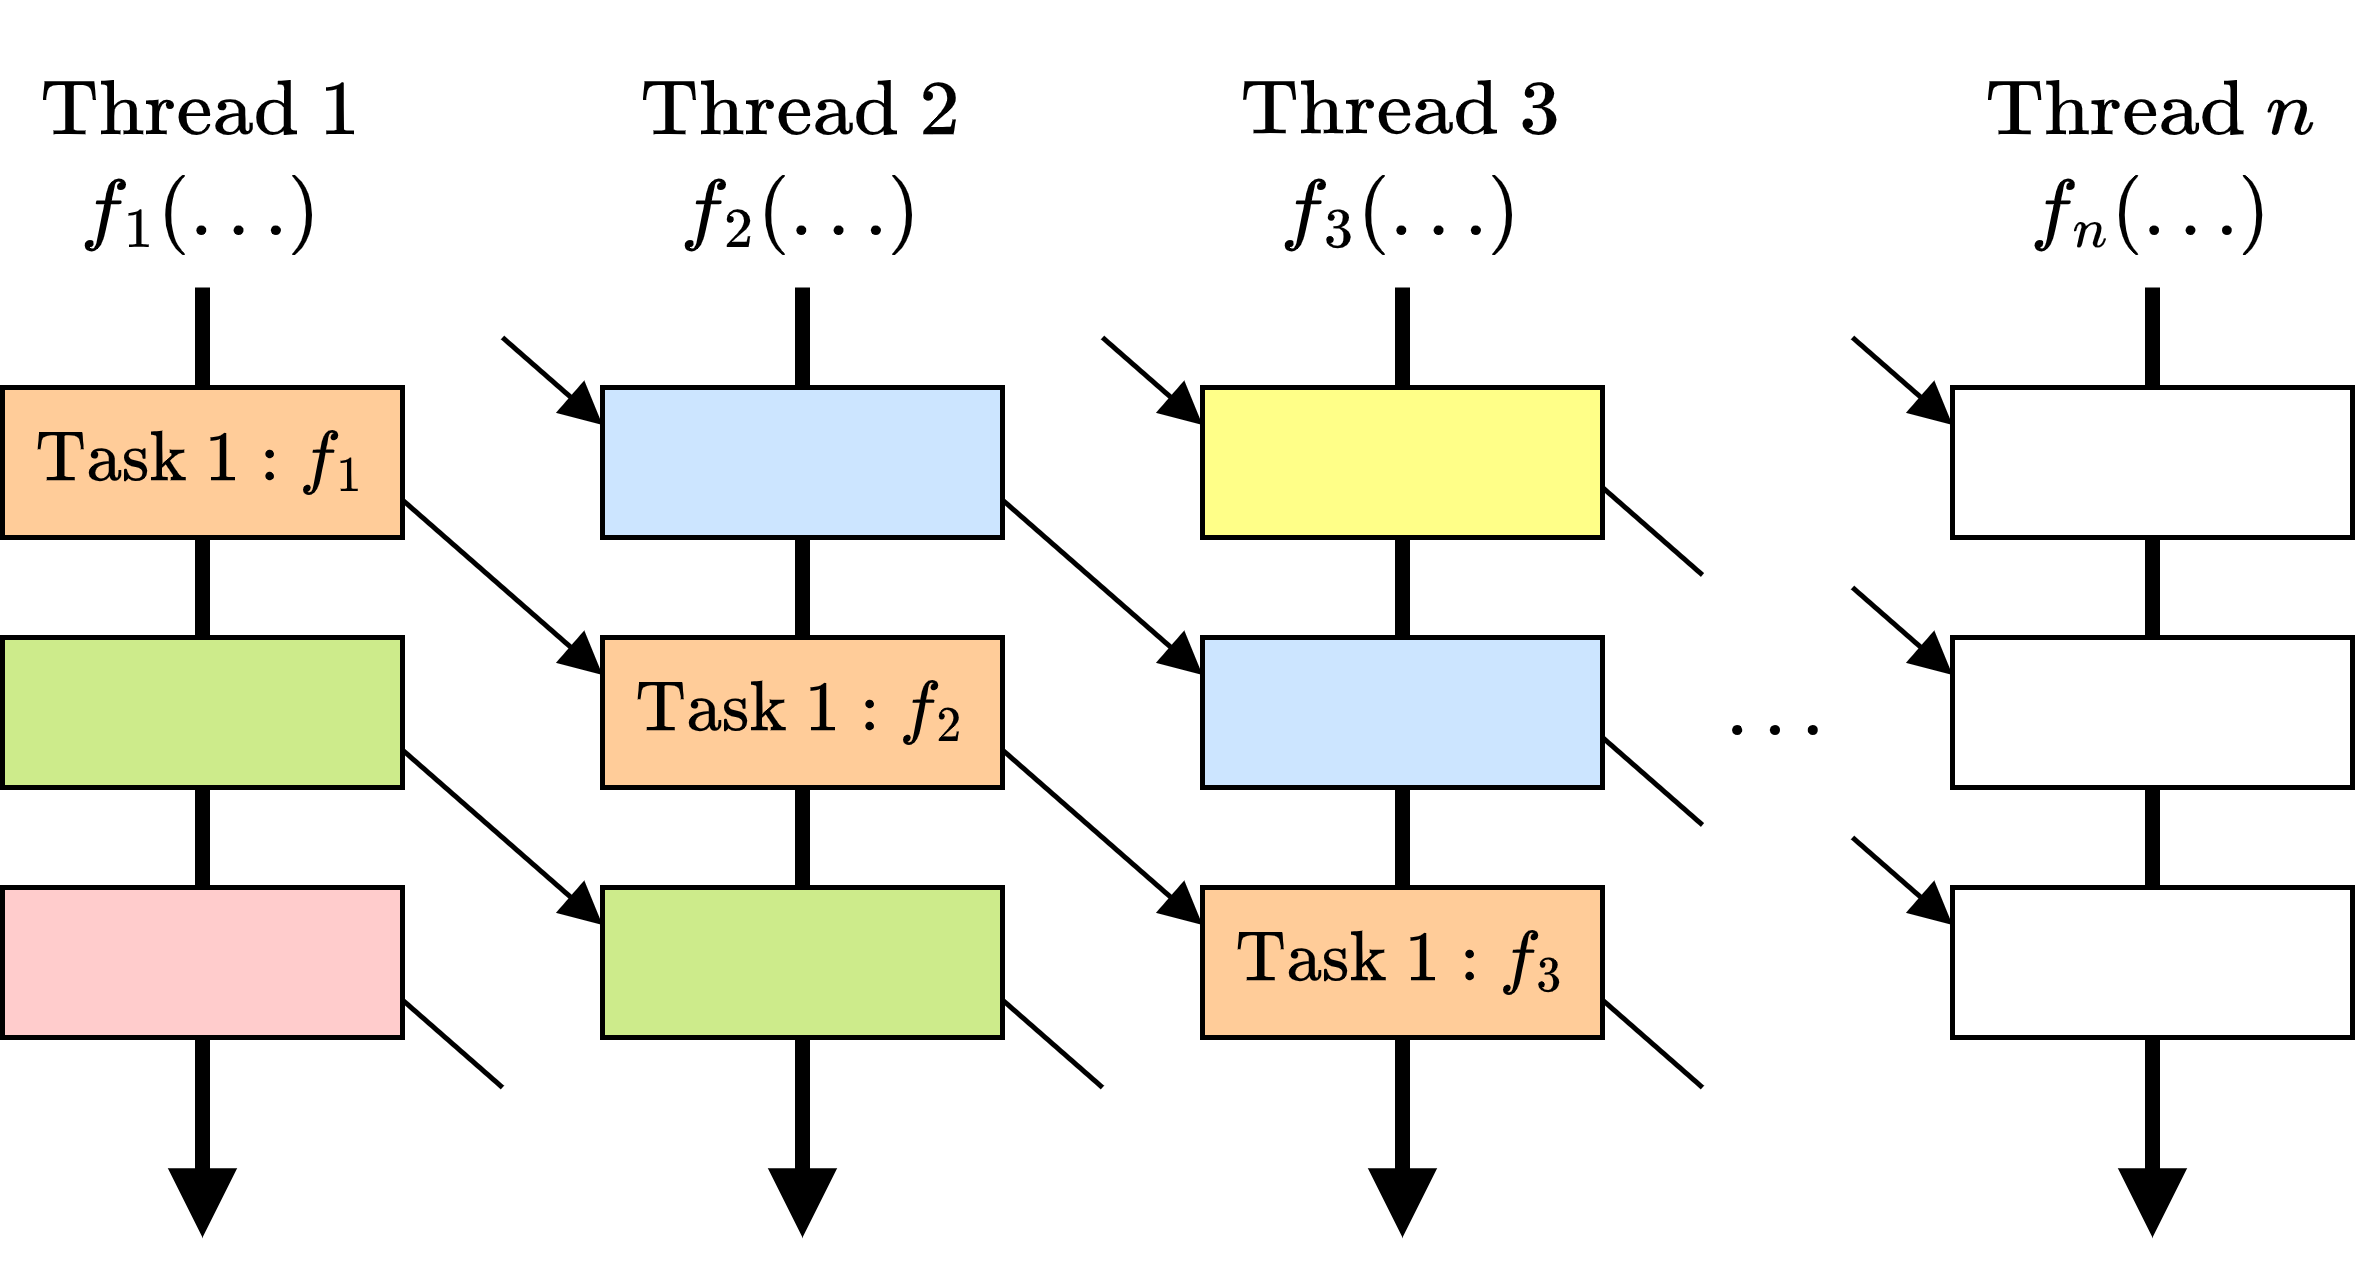
\includegraphics[width=.8\textwidth]{parallelism/images/streaming.drawio.png}
\end{center}
Rather than executing tasks in parallel, execute each stage of a task in a pipeline.
\begin{itemize}
    \item Data needs to be communicated between threads (shared memory between cores)
    \item Temporary data for each stage is not shared.
\end{itemize}
\begin{tabbox}{prosbox}
    \textbf{I-Cache Locality} & Running the same code many times for better temporal locality in instruction cache. \\
\end{tabbox}
\begin{tabbox}{consbox}
    \textbf{D-Cache Locality} & Data must be input and output from stages. Hence we necessarily get slower initial access times due to sharing data \& cache coherency protocol. \\
    \textbf{Pipeline Woes} & Get common issues related to unbalanced pipeline stages/pipeline fragmentation. \\
    \textbf{Flexibility} & If the number of tasks increases of decreases, we cannot just spawn or remove a thread (as with work stealing, dispatch etc), we need to add/remove an entire pipeline. \\ 
\end{tabbox}

\begin{definitionbox}{Staged Event Diven Architecture (SEDA)}
    A combination of streaming and worker-pool based systems.
    \begin{itemize}
        \item Each stage has an input queue, as well as its own thread pool.
        \item When a bottleneck occurs (e.g a queue becomes full) a stage can make a decision (e.g drop a request)
        \item Flexible/can react to load (i.e stages can spawn or remove threads from their pools)
        \item Queues mean stages can be inspected to see contents \& size to optimise for load.
    \end{itemize}
    The \href{https://web.archive.org/web/20120704004128/http://www.eecs.harvard.edu/~mdw/papers/mdw-phdthesis.pdf}{paper behind SEDA} provides a webserver example:
    \begin{center}
        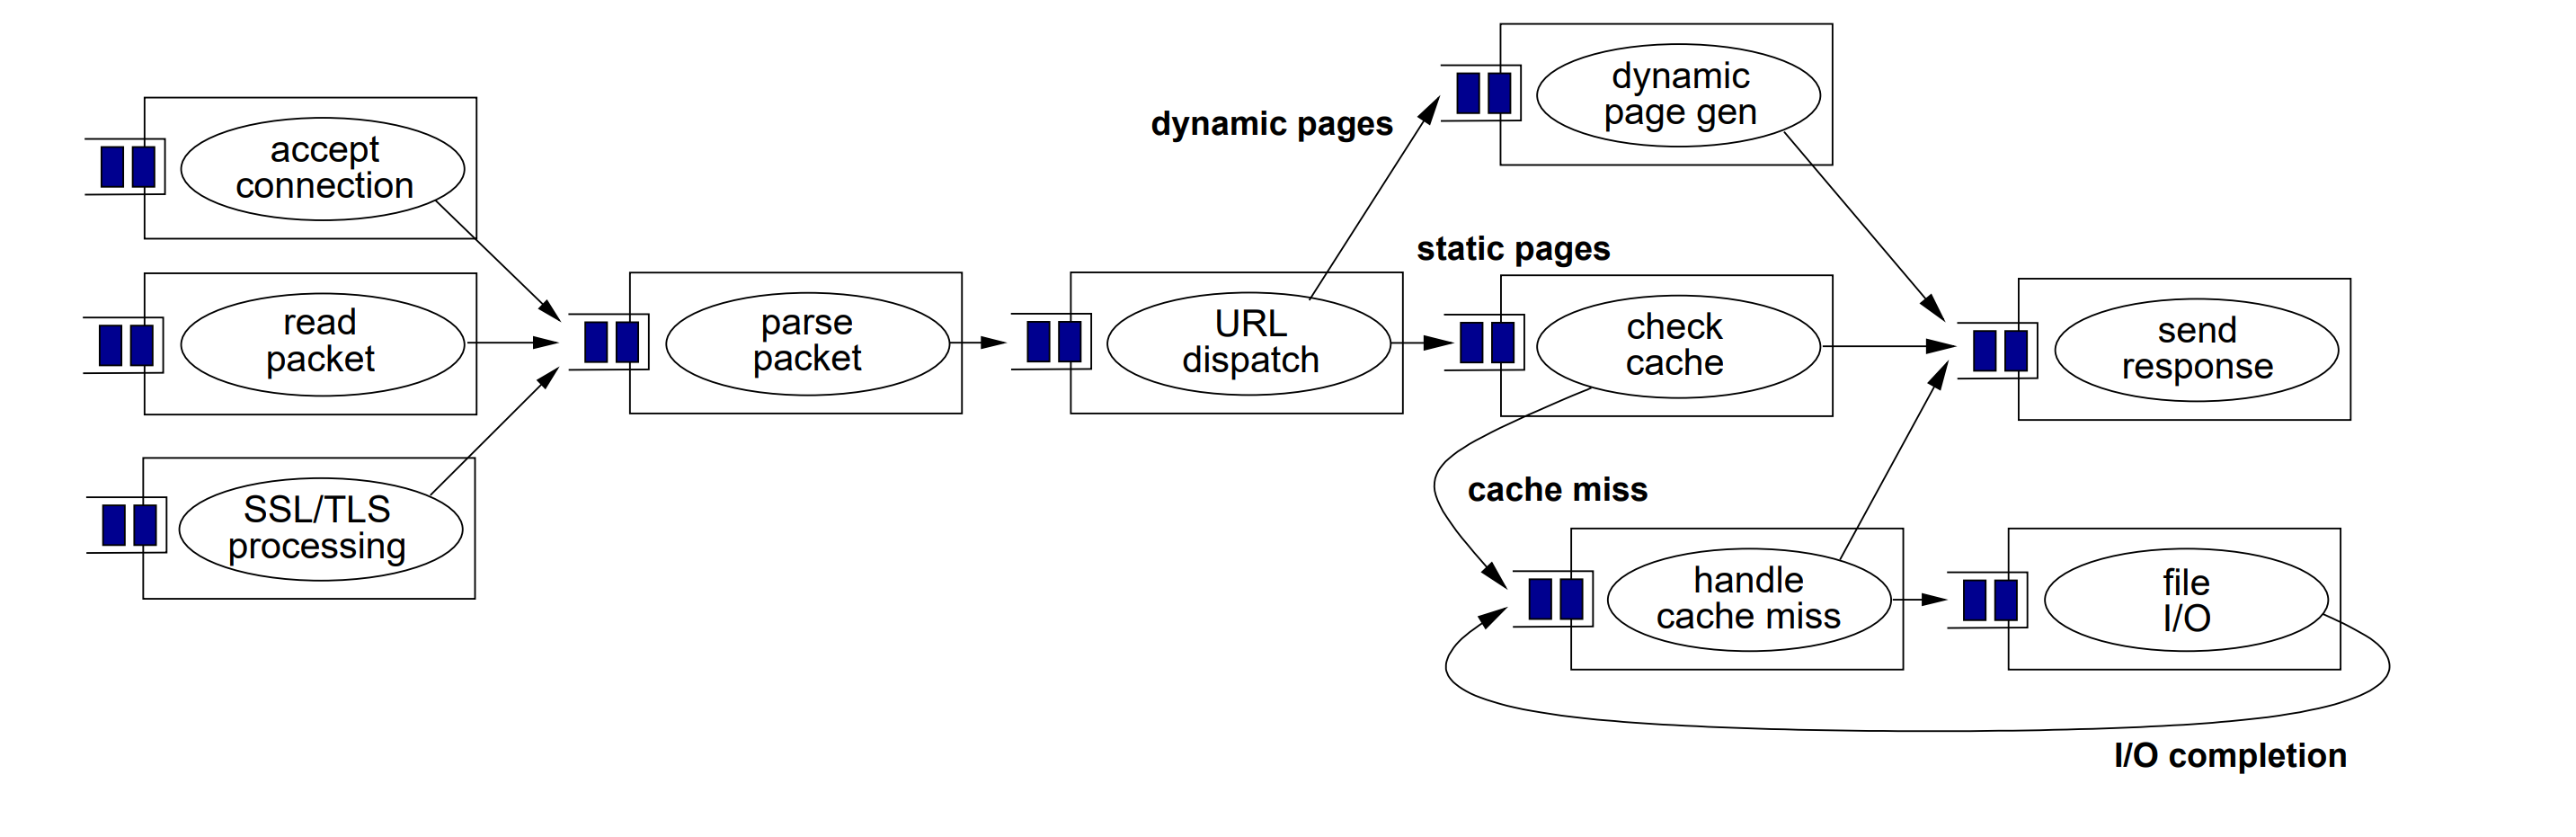
\includegraphics[width=.9\textwidth]{parallelism/images/SEDA.png}
    \end{center}
\end{definitionbox}

\section{Allocators}
A single global allocator is a source of contention in a multithreaded system.
\begin{itemize}
    \item Use a cache of blocks per-thread, this cache can be accessed without contention.
    \item Does global allocation \& free in batches. 
\end{itemize}

\section{Multiprocessing}
\unfinished

\section{Programming Models}
\unfinished
% Thread per task

% Worker Pools


% Event based
% Callbacks
% Futures
% Coroutines
